%
% File acl2018.tex
%
%% Based on the style files for ACL-2017, with some changes, which were, in turn,
%% Based on the style files for ACL-2015, with some improvements
%%  taken from the NAACL-2016 style
%% Based on the style files for ACL-2014, which were, in turn,
%% based on ACL-2013, ACL-2012, ACL-2011, ACL-2010, ACL-IJCNLP-2009,
%% EACL-2009, IJCNLP-2008...
%% Based on the style files for EACL 2006 by 
%%e.agirre@ehu.es or Sergi.Balari@uab.es
%% and that of ACL 08 by Joakim Nivre and Noah Smith

\documentclass[11pt,a4paper]{article}
\usepackage[hyperref]{acl2018}
\usepackage{times}
\usepackage{latexsym}
\usepackage{float}
\usepackage{graphicx}
\graphicspath{ {images/} }

\usepackage{url}

\aclfinalcopy
\newcommand\BibTeX{B{\sc ib}\TeX}

\title{Argument Mining in Wikipedia Articles}

\author{Ben Rothschild \\
  {\tt bnroths@uchicago.edu} \\\And
  Julia Zhou \\
  {\tt juliazhou@uchicago.edu} \\}

\date{}

\begin{document}
\maketitle
\begin{abstract}
  
\end{abstract}

\section{Introduction}
Argumentation mining aims to identify structured argument data from unstructured text.  Applications of argumentation mining are vast and include improving information retrieval from long text, summarizing arguments in legal texts, scientific writing, and news articles or accessing student's command of subject knowledge in essay assignments.  Recently argumentation mining has also been used to develop technologies that can assist humans to debate and reason.  

The task of identifying arguments is difficult though because of the various forms arguments can take in relation to a document or topic.  Part of argumentation mining is also determining if an argument is Pro vs. Con a specific topic.  This is called stance identification and is a difficult NLP task because the subtle nature language can play in taking a stance that often relies on context and subtle word choices or stance development within an argument.  Current approaches are engineered to address specific domains, for example a specific model might be built just to analyze claims in court documents using attributes specific to court documents and legal vocabulary.  However, we believe that argumentative sentences are often characterized by common rhetorical structures, independently of the domain and we propose to explore a method that exploits structured parsing information to detect claims without resorting to topic specific information. 

An example of this would be taking a topic like “the sale of violent video games harms minors” and a wikipedia article about the ​Video game content rating system​ and identifying if a specific sentence or entire text of the article has a Pro or Con stance towards the topic. The article includes the sentence “Exposure to violent video games causes at least a temporary increase in aggression and this exposure correlates with aggression in the real world” which should be labeled as a PRO stance.
There are two main tasks in this problem:
- Identifying claims in text, this will be done through an entity resolution and scoring task
using SVM
- Identifying the stance of a claim against a topic, this will be done similar to a sentiment
classification task
By combining these tasks we will be able to tell what sentences in a long text support and oppose a claim.
\section{Related Work}
\cite{bar2017stance}
LIT REVIEW ANYTHING? (good examples in Roy Bar-Haim paper \\
\section{Data}
The dataset we are using is the Claim Stance Dataset from IBM Debater project which can be accessed here \url{http://www.research.ibm.com/haifa/dept/vst/debating_data.shtml}​.  It contains 2,394 labeled claims for 55 topics that are pulled from 1,065 wikipedia articles.  For each article we are given the following data points:

\begin{itemize}
\item Full text from Wikipedia (tex)
\item Topic Target (text)
\item Claim Text (text)
\item Claim Start Index (integer)
\item Claim End Index (integer)
\item Stance (Pro or Con)
\end{itemize}

The dataset was created by first looking at the list of controversial issues \url{https://en.wikipedia.org/wiki/
Wikipedia:List_of_controversial_issues} Wikipedia identifies to find a subset of 56 topics where there was a clear two-sided debate.  From these topics 546 articles were identified that night have claims in them.  Annotators then read these articles and identified claims and stances within the articles.  An example observation in the dataset would be as follows: \\
\textbf{Full Text} 44,000 words plain text wikipedia article\\
\textbf{Topic Target} the sale of violent video games to minors\\
\textbf{Claim Text} they increase the violent tendencies among youth\\
\textbf{Claim Start Index} 8119\\
\textbf{Claim End Index} 8167\\
\textbf{Stance} PRO\\
Each of the 55 topics was annotated and claims were labeled independently by five annotators.  Some claims were thrown out because of annotator disagreement.  In the final dataset, 98.5\% of the claims had agreement on the claim boundaries and stance.  A full description of the data annotation and collection process can be found here \cite{toledo2016expert}

For each article, the algorithm identifies claims and stance (Pro/Con) towards the topic. Additional fine-grained annotations such as topic target, topic sentiment towards its target, claim target, claim sentiment towards its target, and the relation between the targets are also included based on the semantic model of Bar-Haim et al 

\section{Method Overview}
We divided this research problem into two parts, claim identification and stance identification.
\subsection{Claim Identification}
\subsection{Claim Stance Classification}

Stance classification focuses on the problem of determining if a claim is PRO or CON, a classification stack given by the following function:
\begin{equation}
Stance(c, t)=  sim(c_{sentiment}, t_{sentiment})
\end{equation}

The first hypothesis we have is the following:  Vectors representing the claim and the target were similar then the stance would be PRO and if they very different than the stance would be CON.

In order to test this hypothesis we created word embeddings using Word2Vec and the $gensim$ python package trained on Wikipedia corpus that was used in dataset.  From these embeddings we created a MeanEmbeddingVector which was the mean vector of the list of vectors for the words that represent the sentence.  We trained the model using Logistic Regression and Random Forests.  Similarity between the topic vector and claim vector was measured using cosine similarity.  

\begin{figure}[H]
    \centering
    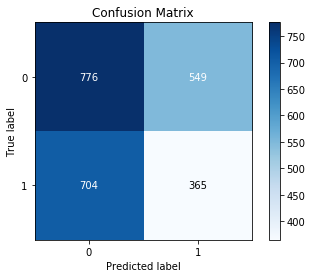
\includegraphics[width=0.35\textwidth]{stance_w2v_lr}
    \caption{\label{font-table} Confusion Matrix for Logistic Model }
\end{figure} 

\begin{figure}[H]
    \centering
    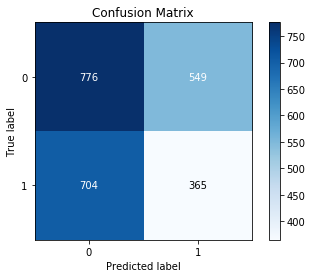
\includegraphics[width=0.35\textwidth]{stance_w2v_lr}
    \caption{\label{font-table} Confusion Matrix for Random Forest }
\end{figure} 

Below are the accuracy and loss of the model trained and reported using a stratified cross-validation with three folds.
StratifiedKFold
\begin{table}[H]
\begin{center}
\begin{tabular}{|c|c|c|}
\hline \bf & \bf Log Loss & \bf Accuracy \\ \hline
Logistic & 1.15 & 47.6 \\
Random Forests & .809 & 47.5 \\
\hline
\end{tabular}
\end{center}
\end{table}

Considering there are only two classes, this accuracy is very bad and we aren't able to determine better than chance at the stance of a specific claim.  The code for this section is 4\_stance\_detection.ipynb

The next hypothesis we had is that instead of containing similar words or sentence embeddings, claims and targets can be classified by using their sentiment.  The hypothesis would be as follows:  Claim that have a similar sentiment as a topic will be PRO and divergent sentiment will be CON.  This idea is summarized in the following table:

\begin{table}[H]
\begin{center}
\begin{tabular}{|c|c|c|}
\hline \bf & \bf $Claim_{+}$ & \bf $Claim_{-}$ \\ \hline
$Topic_{+}$ & PRO & CON \\
$Topic_{-}$ & CON & PRO \\
\hline
\end{tabular}
\end{center}
\end{table}

To quickly test this hypothesis we will use a pre-trained sentiment analysis model $Vader$ so that we don't have to label our text and train the model ourselves.  We find the positive, negative and neutral sentiment for each sentence and use these to form a vector which calculate the similarity using cosine similiarty.  The confusion matrix is below:
\begin{figure}[H]
    \centering
    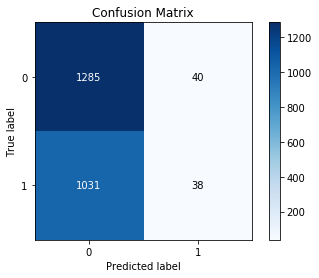
\includegraphics[width=0.35\textwidth]{sentiment_lr}
    \caption{\label{font-table} Confusion Matrix for Logistic Model }
\end{figure} 


Loss and accuracy are calculated similar to as before:

\begin{table}[H]
\begin{center}
\begin{tabular}{|c|c|c|}
\hline \bf & \bf Log Loss & \bf Accuracy \\ \hline
Logistic & .687 & 55.2 \\
Random Forests & .809 & 47.5 \\
\hline
\end{tabular}
\end{center}
\end{table}

\section{Results and Analysis}
\section{Conclusion}


% include your own bib file like this:
%\bibliographystyle{acl}
%\bibliography{acl2018}
\bibliography{acl2018}
\bibliographystyle{acl_natbib}

\end{document}
